\documentclass{article}

\usepackage{csquotes}
% 使用中文CJK包
\usepackage{CJK}
% 图像插入宏包
\usepackage{graphicx}
% 自定义颜色支持
\usepackage[usenames,dvipsnames]{color}
% 长表格跨页支持
\usepackage{longtable}
% 代码高亮支持
\usepackage{listings}
% 算法伪代码包
\usepackage[ruled,vlined]{algorithm2e}
% 自定义标题格式
\usepackage{titlesec}
% 扩展tabular样式
\usepackage{array}
% 添加页眉页脚
\usepackage{fancyhdr}
% 虚拟正文测试
\usepackage{lipsum}
% 数学环境包
\usepackage{amsmath}
% 首行缩进
\usepackage{indentfirst}
% 树状结构图
\usepackage{tree-dvips}
% 脚注环境
\usepackage{footnote}
% 定制表格线
\usepackage{makecell}
% tikz绘图包
\usepackage{tikz}
% URL超链接
\usepackage[dvips, colorlinks, linkcolor=black]{hyperref}
% 断行URL超链接
\usepackage{breakurl}


% hyperref中文兼容
\pdfstringdefDisableCommands{
\let\CJK@XX\relax
\let\CJK@XXX\relax
\let\CJK@XXXp\relax
\let\CJK@XXXX\relax
\let\CJK@XXXXp\relax
}

\usetikzlibrary{positioning,shapes,shadows,arrows}


% 设置脚注在table中可用
\makesavenoteenv{table}

% 设置标题格式
%\titleformat{\chapter}{\raggedright\Huge\bfseries}{Chapter \thechapter}{1em}{}

% 设置默认字体族, 具体字体请查看texdoc psnfss2e

% 设置Roman字体为Palatino
\renewcommand{\rmdefault}{ppl} 
% 设置TypeWriter字体为Courier
\renewcommand{\ttdefault}{pcr} 

% 设置行距
\setlength{\parskip}{1ex}

% 定义需要的颜色

\definecolor{lightgray}{RGB}{230,230,230}
\definecolor{lightblue}{RGB}{224, 224, 255}
\definecolor{darkblue}{RGB}{192, 192, 255}
\definecolor{lightpink}{RGB}{255, 224, 224}
\definecolor{darkpink}{RGB}{255, 192, 192}
\definecolor{keywordyellow}{RGB}{255, 204, 0}
\definecolor{keywordred}{RGB}{194, 58, 0}
\definecolor{numbercolor}{RGB}{102, 51, 0}

% 设置代码风格

% 定义C语言代码风格
\lstdefinestyle{ccode}
{ 
    language=C, 
    numbers=left, 
    numberstyle=\color{numbercolor},
    basicstyle=\scriptsize\ttfamily\bfseries,
    keywordstyle=\color{blue}, 
    commentstyle=\color{PineGreen},
    stringstyle=\color{red}, 
    frame=shadowbox, 
    frameround=tttt,
    breaklines=true,
    backgroundcolor=\color{lightgray} }

% 定义汇编语言代码风格
\lstdefinestyle{acode}
{ 
    language=,
    morekeywords=[1]{mov, movl, movb, movw, orl, xorw, cli, cld, inb, testb, test, jnz, push, pop, jmp, call, lea, add, sub, ret, jle, outb, ljmp, lgdt},
    morekeywords=[2]{ax, bx, cx, dx, eax, ebx, ecx, edx, cr0, cr1, cr2, cr3, al, ds, es, ss, esp, ebp}, 
    morekeywords=[3]{data, text, bss},
    morekeywords=[4]{long, align, p2align, ascii, fill, globl, space, set, rept, byte, word},
    morecomment=[l]\#,
    numbers=left, 
    numberstyle=\color{numbercolor},
    basicstyle=\scriptsize\ttfamily\bfseries,
    keywordstyle=[1]\color{blue}, 
    keywordstyle=[2]\color{keywordyellow},
    keywordstyle=[3]\color{orange},
    keywordstyle=[4]\color{keywordred},
    commentstyle=\color{PineGreen},
    stringstyle=\color{red}, 
    frame=shadowbox, 
    frameround=tttt,
    breaklines=true,
    backgroundcolor=\color{lightgray} }

    
% 定义命令行输出风格
\lstdefinestyle{console}
{
    language=bash, 
    numbers=none, 
    frame=tRBl,
    basicstyle=\scriptsize\color{green}\ttfamily\bfseries,     
    backgroundcolor=\color{black}}


% 定义exercise输出风格
\lstdefinestyle{exercise}
{
    numbers=none, 
    frame=tRBl,
    breaklines=true,
    breakindent=0pt,
    framexleftmargin=1em,
    framexrightmargin=1em,
    framextopmargin=2ex,
    framexbottommargin=2ex,
    xleftmargin=0.05\linewidth,
    xrightmargin=0.05\linewidth,
    basicstyle=\scriptsize\ttfamily\mdseries,   
    moredelim=[is][\ttfamily\bfseries]{|}{|},
    framerule=0.8pt,
    rulecolor=\color{darkblue}, 
    backgroundcolor=\color{lightblue}}
    

% 定义challenge输出风格
\lstdefinestyle{challenge}
{
    numbers=none, 
    frame=tRBl,
    breaklines=true,
    breakindent=0pt,
    framexleftmargin=1em,
    framexrightmargin=1em,
    framextopmargin=2ex,
    framexbottommargin=2ex,
    xleftmargin=0.05\linewidth,
    xrightmargin=0.05\linewidth,
    basicstyle=\scriptsize\ttfamily\mdseries,   
    moredelim=[is][\ttfamily\bfseries]{|}{|},
    framerule=0.8pt,
    rulecolor=\color{darkpink}, 
    backgroundcolor=\color{lightpink}}
    


% 非常重要, listings关闭非ASCII字符兼容
\lstset{extendedchars=false}


% 定义问题的答案格式
\newcommand{\highlight}[1]{{\bfseries \color{red}  #1}}
% 定义函数名格式
\newcommand{\funcname}[1]{{\ttfamily \small #1}}




\pagestyle{fancy}
\begin{document}
\begin{CJK*}{UTF8}{gkai}

\lhead{操作系统实习报告}
\rhead{张弛, 00848231}
\title{操作系统JOS实习第二次报告}
\author{张弛 \hspace{1ex} 00848231, \\
        zhangchitc@gmail.com}

\maketitle
% 记得在文档末尾插入\clearpage
\tableofcontents
\newpage

\section{Introduction}

我在实验中主要参考了华中科技大学邵志远老师写的JOS实习指导,在邵老师的主页上\burl{http://grid.hust.edu.cn/zyshao/OSEngineering.htm} 可以找到。但是这次实验的指导远远不如lab1的指导详尽,所以我这里需要补充的内容会很多。

\section{Physical Page Management}


\begin{lstlisting}[style=exercise]
|Exercise 1|. In the file kern/pmap.c, you must implement code for the following functions.

        boot_alloc()
	page_init()
	page_alloc()
	page_free()
	
You also need to add some code to i386_vm_init() in pmap.c, as indicated by comments there. For now, just add the code needed leading up to the call to check_page_alloc().

You probably want to work on boot_alloc(), then i386_vm_init(), then page_init(), page_alloc(), and page_free().

check_page_alloc() tests your physical page allocator. You should boot JOS and see whether check_page_alloc() reports success. Fix your code so that it passes. You may find it helpful to add your own assert()s to verify that your assumptions are correct.
\end{lstlisting}

这部分实验的内容暂时和页面转换机制没有关系,我们需要重点关注的是物理页面的规划以及管理。主要需要关注JOS内核代码中的inc/queue.h文件以及kern/pmap.c文件。

\subsection{Physical page and its data structure}

请仔细阅读邵老师的讲义中4.3章 第一节 页面管理。其中重点需要掌握以下内容:

\begin{enumerate}
\item{物理页和Page数据结构的对应关系}
\item{对Page*页面链表的宏操作,在inc/queue.h中}
\end{enumerate}

里面我唯一碰到的问题就是没看懂为什么JOS给出的链表模板要写成下面这样的形式:

\begin{lstlisting}[style=ccode, firstnumber=165, title={\scriptsize \ttfamily \bfseries inc/queue.h}]
/*
 * Reset the list named "head" to the empty list.
 */
#define	LIST_INIT(head) do {						\
	LIST_FIRST((head)) = NULL;					\
} while (0)
\end{lstlisting}

这个宏的的目的是将链表初始化为空。但我奇怪的是为什么要写成一个只执行一次的while循环的形式,而不是直接大括号包住这一段语句就可以了? 实验室的白光东师兄给出了一个详尽满意的答案。他给了我下面这样的程序:

\begin{lstlisting}[style=ccode, title={\scriptsize \ttfamily \bfseries test.c}]
#include <stdio.h>

#define MACRO() do { \
  printf ("hello\n"); \
} while (0)

int main () {
  int x;
  scanf ("%d\n", &x);

  if (x) 
    MACRO ();
  else
    printf ("this is else\n");
  return 0;
}
\end{lstlisting}

然后使用gcc -E test.c编译这段程序,参数E的目的是为了让编译器仅仅进行预编译以后即停下来,并输出预编译后的程序结果,那么我们得到这样的输出

\begin{lstlisting}[style=console]
int main () {
  int x;
  scanf ("%d\n", &x);

  if (x)
    do { printf ("hello\n"); } while (0);
  else
    printf ("this is else\n");
  return 0;
}
zhangchi@zhangchi-desktop:/tmp/test$ 
\end{lstlisting}

很明显我们看到相关的\funcname{MACRO ();}调用变成了其相应的宏展开,请特别注意,调用的时候我们是以单个语句的形式调用\funcname{MACRO ()}的,那么展开以后的形式还是满足了单个语句(一个while循环),并且,在其后面加上了分号。如果我们把MACRO改成:

\begin{lstlisting}[style=ccode, title={\scriptsize \ttfamily \bfseries test.c}]
#define MACRO() { \
  printf ("hello\n"); \
}
\end{lstlisting}

那么再次展开的结果会变成:


\begin{lstlisting}[style=console]
int main () {
  int x;
  scanf ("%d\n", &x);

  if (x)
    { printf ("hello\n"); };
  else
    printf ("this is else\n");
  return 0;
}
zhangchi@zhangchi-desktop:/tmp/test$ 
\end{lstlisting}

明显可以看出这样的转换造成语法错误,用大括号包裹的代码块后不需要分号。这里出错的原因就在于我们调用\funcname{MACRO ()}之前是当成一个单个语句,调用展开后变成了一个代码块。那么相应的语法结构就出现了变化导致出错。

真是考虑得非常细致!感谢师兄!

\subsection{Physical memory layout}

请仔细阅读邵老师的讲义中的4.3章 第一节 页面管理 中``页面管理链表在内存中的存储和放置''小节。重点理解

\begin{enumerate}
\item{pages数组和Page*链表的对应关系}
\item{pages所在的空间是怎样分配的}
\item{整个物理内存的布局}
\end{enumerate}

这里要说的是,在做完lab1以后,我们知道了在实模式下物理页面前640KB的一些分配情况,如BIOS的载入地址、boot loader载入地址、操作系统内核ELF文件头的临时存放空间等等,具体的布局应该如下图所示:

\begin{figure}[htp]
\centering
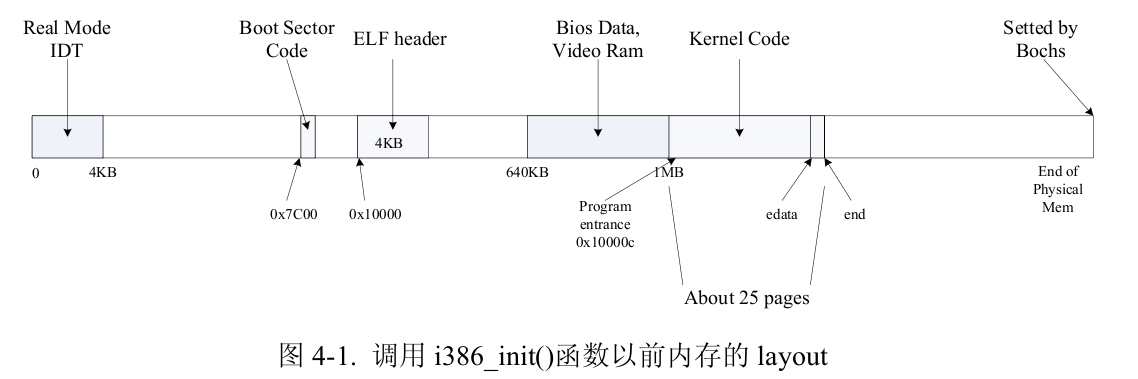
\includegraphics[scale=0.320]{/home/zhangchi/lab/report/screen1.png}
\end{figure}

在lab1完成后,我们从0x000100000这个位置放入内核,直到end结束。end是链接器作链接时得到的内核结束地址。

那么在建立物理页面对应的Page* 链表时,我们需要为这个链表分配实际的物理内存空间,在二级页地址映射机制中,系统还需要一个页目录存下所有二级页表的地址,这个也是需要操作系统预先分配空间的,所以结合上图,我们第一步完成之后物理内存布局应该如下图所示:


\begin{figure}[htp]
\centering
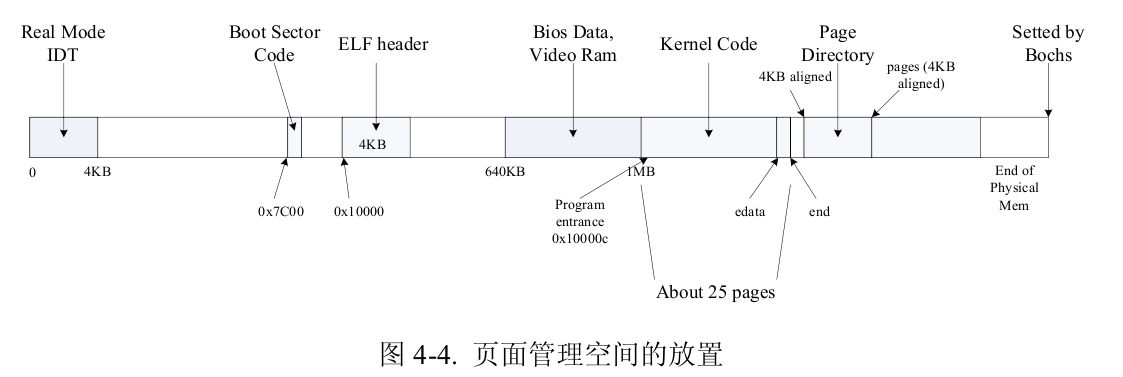
\includegraphics[scale=0.320]{/home/zhangchi/lab/report/screen2.png}
\label{physmemlayout}
\end{figure}

我们第一步的目的就是为页目录和pages分配好空间,并建立起空闲页表page\_free\_list。


开始写代码的时候,首先需要弄清楚kern/pmap.c中的几个基本的变量:

\begin{lstlisting}[style=ccode, firstnumber=12, title={\scriptsize \ttfamily \bfseries kern/pmap.c}]
// These variables are set by i386_detect_memory()
static physaddr_t maxpa;	// Maximum physical address
size_t npage;			// Amount of physical memory (in pages)
static size_t basemem;		// Amount of base memory (in bytes)
static size_t extmem;		// Amount of extended memory (in bytes)

// These variables are set in i386_vm_init()
pde_t* boot_pgdir;		// Virtual address of boot time page directory
physaddr_t boot_cr3;		// Physical address of boot time page directory
static char* boot_freemem;	// Pointer to next byte of free mem

struct Page* pages;		// Virtual address of physical page array
static struct Page_list page_free_list;	// Free list of physical pages
\end{lstlisting}

这里只需要知道两个变量,boot\_freemem和boot\_pgdir,前者是当前可用内存的开始地址(也就是说,内核载入以后,系统管理所需要的内容就从end以后开始分配,即从一开始boot\_freemem是等于end,这个在接下来的代码里就能看到);boot\_pgdir则是系统页目录所在空间的开始地址。\highlight{注意,两者地址都是虚拟地址!在这次lab中一定要搞清楚的一个细节就是虚拟地址,线性地址和物理地址的区别,以及我们使用的地址变量哪些是虚拟地址,哪些是物理地址。}


接下来我们可以看到\funcname{i386\_vm\_init ()},从这里开始我们这次的lab。一开始就看到关于页目录的初始化代码:

\begin{lstlisting}[style=ccode, title={\scriptsize \ttfamily \bfseries kern/pmap.c: i386\_vm\_init ()}]
	//////////////////////////////////////////////////////////////////////
	// create initial page directory.
	pgdir = boot_alloc(PGSIZE, PGSIZE);

	memset(pgdir, 0, PGSIZE);
	boot_pgdir = pgdir;
	boot_cr3 = PADDR(pgdir);
\end{lstlisting}

其中\funcname{boot\_alloc ()}为其分配内存空间地址,然后将分配的地址段清空。然后将其物理地址(PADDR)放入boot\_cr3准备启动x86的页面地址转换机制。这里要注意几点:

\begin{itemize}
\item{PGSIZE为一个物理页的大小4KB = 4096B,定义在inc/mmu.h中,其中还有我们后面要用的重要常量PTSIZE,为一个页表对应实际物理内存的大小,即1024 * 4KB = 4MB}
\item{从\funcname{boot\_alloc ()}得到的页面是不会作相应的初始化工作的,所以如果对分配到的空间有要求清空,必须自己亲自动手}
\item{\funcname{memset}接受的清空地址是pgdir即一个虚拟地址,这个在我们后面的工作中对实际分配到的\highlight{物理页面}进行初始化时提醒,清空时使用\funcname{memset}也一定要使用实际物理页面对应的\highlight{内核虚拟地址}}
\item{boot\_cr3得到的是一个\highlight{物理地址},这个和我们前面强调的分清每个地址变量到底是虚拟地址还是物理地址有密切联系}
\end{itemize}

接下来我们来看一下第一个需要实现的函数\funcname{boot\_alloc ()}

\begin{lstlisting}[style=ccode, title={\scriptsize \ttfamily \bfseries kern/pmap.c: boot\_alloc ()}]
static void*
boot_alloc(uint32_t n, uint32_t align)
{
	extern char end[];
	void *v;

	// Initialize boot_freemem if this is the first time.
	// 'end' is a magic symbol automatically generated by the linker,
	// which points to the end of the kernel's bss segment -
	// i.e., the first virtual address that the linker
	// did _not_ assign to any kernel code or global variables.
	if (boot_freemem == 0)
		boot_freemem = end;

	// LAB 2: Your code here:
	//	Step 1: round boot_freemem up to be aligned properly
	//		(hint: look in types.h for some handy macros)
	//	Step 2: save current value of boot_freemem as allocated chunk
	//	Step 3: increase boot_freemem to record allocation
	//	Step 4: return allocated chunk

    	v = ROUNDUP (boot_freemem, align);
    	boot_freemem = (char*) v + n;
    
	return v;
}
\end{lstlisting}

这个函数的问题不大。

看接下来的代码:\label{vpt}

\begin{lstlisting}[style=ccode, title={\scriptsize \ttfamily \bfseries kern/pmap.c: i386\_vm\_init ()}]
	//////////////////////////////////////////////////////////////////////
	// Recursively insert PD in itself as a page table, to form
	// a virtual page table at virtual address VPT.
	// (For now, you don't have understand the greater purpose of the
	// following two lines.)

	// Permissions: kernel RW, user NONE
	pgdir[PDX(VPT)] = PADDR(pgdir)|PTE_W|PTE_P;

	// same for UVPT
	// Permissions: kernel R, user R 
	pgdir[PDX(UVPT)] = PADDR(pgdir)|PTE_U|PTE_P;

	//////////////////////////////////////////////////////////////////////
	// Allocate an array of npage 'struct Page's and store it in 'pages'.
	// The kernel uses this array to keep track of physical pages: for
	// each physical page, there is a corresponding struct Page in this
	// array.  'npage' is the number of physical pages in memory.
	// User-level programs will get read-only access to the array as well.
	// Your code goes here:
	

	pages = boot_alloc (npage * sizeof (struct Page), PGSIZE);

	//////////////////////////////////////////////////////////////////////
	// Now that we've allocated the initial kernel data structures, we set
	// up the list of free physical pages. Once we've done so, all further
	// memory management will go through the page_* functions. In
	// particular, we can now map memory using boot_map_segment or page_insert
	page_init();

	check_page_alloc();

	page_check();
\end{lstlisting}

前两句对pgdir的操作我们可以先不用管他,在后来设置页表的时候我们会回过头来看这两句话的含义。在23行里为pages分配空间以后,就进入倒\funcname{page\_init ()}对链表进行初始化了。

在进行接下来的编码之前,我们先需要了解JOS对于地址编码的一些规定,在inc/mmu.h中,我们可以找到一组详尽的宏:

\begin{lstlisting}[style=ccode, firstnumber=16, title={\scriptsize \ttfamily \bfseries inc/mmu.h}]
// A linear address 'la' has a three-part structure as follows:
//
// +--------10------+-------10-------+---------12----------+
// | Page Directory |   Page Table   | Offset within Page  |
// |      Index     |      Index     |                     |
// +----------------+----------------+---------------------+
//  \--- PDX(la) --/ \--- PTX(la) --/ \---- PGOFF(la) ----/
//  \----------- PPN(la) -----------/
//
// The PDX, PTX, PGOFF, and PPN macros decompose linear addresses as shown.
// To construct a linear address la from PDX(la), PTX(la), and PGOFF(la),
// use PGADDR(PDX(la), PTX(la), PGOFF(la)).

// page number field of address
#define PPN(la)		(((uintptr_t) (la)) >> PTXSHIFT)
#define VPN(la)		PPN(la)		// used to index into vpt[]

// page directory index
#define PDX(la)		((((uintptr_t) (la)) >> PDXSHIFT) & 0x3FF)
#define VPD(la)		PDX(la)		// used to index into vpd[]

// page table index
#define PTX(la)		((((uintptr_t) (la)) >> PTXSHIFT) & 0x3FF)

// offset in page
#define PGOFF(la)	(((uintptr_t) (la)) & 0xFFF)

// construct linear address from indexes and offset
#define PGADDR(d, t, o)	((void*) ((d) << PDXSHIFT | (t) << PTXSHIFT | (o)))
\end{lstlisting}


其中PDX,PTX和PGOFF都很好理解,需要注意的是PPN,一个\highlight{线性地址}的PPN其实没有什么意义,但是如果我们对一个\highlight{物理地址}取PPN的话,就可以利用这个PPN直接访问\highlight{这个物理地址在pages数组中的对应页}!这个宏所以非常的好用。

我们来看到前面提到对物理页面链表进行初始化的\funcname{page\_init ()} 过程:



\begin{lstlisting}[style=ccode, title={\scriptsize \ttfamily \bfseries kern/pmap.c: boot\_init ()}]
//
// Initialize page structure and memory free list.
// After this is done, NEVER use boot_alloc again.  ONLY use the page
// allocator functions below to allocate and deallocate physical
// memory via the page_free_list.
//
void
page_init(void)
{
    // The example code here marks all physical pages as free.
    // However this is not truly the case.  What memory is free?
    //  1) Mark physical page 0 as in use.
    //     This way we preserve the real-mode IDT and BIOS structures
    //     in case we ever need them.  (Currently we don't, but...)
    //  2) The rest of base memory, [PGSIZE, basemem) is free.
    //  3) Then comes the IO hole [IOPHYSMEM, EXTPHYSMEM).
    //     Mark it as in use so that it can never be allocated.
    //  4) Then extended memory [EXTPHYSMEM, ...).
    //     Some of it is in use, some is free. Where is the kernel
    //     in physical memory?  Which pages are already in use for
    //     page tables and other data structures?
    //
    // Change the code to reflect this.
    //

    int i;
    int lower_ppn = PPN (IOPHYSMEM);
    int upper_ppn = PPN (ROUNDUP (boot_freemem, PGSIZE));

    LIST_INIT(&page_free_list);
    for (i = 0; i < npage; i++) {
        pages[i].pp_ref = 0;

        if (i == 0) continue;
        if (lower_ppn <= i && i < upper_ppn) continue;
 
        LIST_INSERT_HEAD(&page_free_list, &pages[i], pp_link);
    }
}
\end{lstlisting}

这个函数的具体工作就是建立其每个物理页面对应的实际链表节点,然后把那些被操作系统占用或是系统预留空间从链表里去除掉。通过对照\ref{physmemlayout}中提到的物理内存的使用布局,可以总结出以下几个使用的物理地址区域:


\begin{description}
\item[$[0, \mathrm{PGSIZE})$] :\newline
存放中断向量表IDT以及BIOS的相关载入程序
\item[$[\mathrm{IOPHYSMEM}, \mathrm{EXTPHYSMEM})$]:\newline
存放输入输出所需要的空间,比如VGA的一部分显存直接映射这个地址
\item[$[\mathrm{EXTPHYSMEM}, \mathrm{end})$]:\newline
存放操作系统内核kernel
\item[$[\mathrm{PADDR(boot\_pgdir)}, \mathrm{PADDR(boot\_pgdir) + \mathrm{PGSIZE}})$]:\newline
存放页目录
\item[$[\mathrm{PADDR(pages)}, \mathrm{boot\_freemem})$]:\newline
存放pages数组
\end{description}

但是除了第一项之外,后面的4段区域实际上是一段连续内存$[\mathrm{IOPHYSMEM}, \mathrm{boot\_freemem})$,所以上面的代码在实现时,把这段区域对应的物理页下标算出来,那么如果是第一个物理页或者是上面区间内的物理页,就不加入空闲页链表里。

接下来我们还要完成两个的对物理页链表的操作:申请和释放,先来看申请的操作\funcname{page\_alloc ()}

\begin{lstlisting}[style=ccode, title={\scriptsize \ttfamily \bfseries kern/pmap.c: page\_alloc ()}]
int
page_alloc(struct Page **pp_store)
{
    // Fill this function in
 	
    if (!LIST_EMPTY (&page_free_list)) {
        *pp_store = LIST_FIRST (&page_free_list);
        LIST_REMOVE (LIST_FIRST (&page_free_list), pp_link);
        return 0;
    }

    return -E_NO_MEM;
}
\end{lstlisting}

这个很简单,直接按照注释来做即可。再看释放页面的\funcname{page\_free ()}

\begin{lstlisting}[style=ccode, title={\scriptsize \ttfamily \bfseries kern/pmap.c: page\_free ()}]
void
page_free(struct Page *pp)
{
    // Fill this function in
	
    LIST_INSERT_HEAD (&page_free_list, pp, pp_link);
}\end{lstlisting}

好像更简单了\ldots好吧亚

这个时候我们重新编译内核后启动JOS,应该可以通过\funcname{check\_page\_alloc() }的所有测试了。

\section{Virtual Memory}


\begin{lstlisting}[style=exercise]
|Exercise 2|. Read chapters 5 and 6 of the Intel 80386 Reference Manual, if you haven't done so already. You can skip 6.3. Although JOS relies most heavily on page translation, you will also need a basic understanding of how segmentation works in protected mode to understand what's going on in JOS.
\end{lstlisting}

貌似我没怎么看\ldots,这个部分的lab请仔细阅读绍老师课件里4.3中第二小节``页表管理''。

\subsection{Virtual, Linear, and Physical Addresses}

\begin{lstlisting}[style=exercise]
|Exercise 3|. While GDB can only access QEMU's memory by virtual address, it's often useful to be able to inspect physical memory while setting up virtual memory. Review the QEMU monitor commands, especially the xp command, which lets you inspect physical memory. To access the QEMU monitor, press Ctrl-a c in the terminal (the same binding returns to the serial console).

Use the xp command in the QEMU monitor and the x command in GDB to inspect memory at corresponding physical and virtual addresses and make sure you see the same data.

QEMU's info mem command may also prove useful in the lab. We've also added an info pg command to our patched version of QEMU that prints out the current page table.
\end{lstlisting}

这里提到的调试命令貌似都没用到过。不过这一章里提到用两种数据类型来区分虚拟和物理地址。这样在我们编写程序时通过函数内部的声明能够很清晰的看出对应操作的地址是哪一类,以便于我们理解代码。

这里提到的有关地址类型的问题

\begin{lstlisting}[style=exercise]
|Question|

|1.| Assuming that the following JOS kernel code is correct, what type should variable x have, uintptr_t or physaddr_t?

	mystery_t x;
	char* value = return_a_pointer();
	*value = 10;
	x = (mystery_t) value;
\end{lstlisting}

因为在内核中操作数据都是以内核虚拟地址进行的,所以x的类型应该是\funcname{uintptr\_t}


\subsection{Reference counting}

从这里就开始提到虚拟内存空间了。里面出现了\funcname{UTOP}这样的地址,那么我们来看看详细定义在inc/memlayout.h中的虚拟内存布局:

\begin{lstlisting}[style=ccode, title={\scriptsize \ttfamily \bfseries inc/memlayout.h}]
/*
 * Virtual memory map:                                Permissions
 *                                                    kernel/user
 *
 *    4 Gig -------->  +------------------------------+
 *                     |                              | RW/--
 *                     ~~~~~~~~~~~~~~~~~~~~~~~~~~~~~~~~
 *                     :              .               :
 *                     :              .               :
 *                     :              .               :
 *                     |~~~~~~~~~~~~~~~~~~~~~~~~~~~~~~| RW/--
 *                     |                              | RW/--
 *                     |   Remapped Physical Memory   | RW/--
 *                     |                              | RW/--
 *    KERNBASE ----->  +------------------------------+ 0xf0000000
 *                     |  Cur. Page Table (Kern. RW)  | RW/--  PTSIZE
 *    VPT,KSTACKTOP--> +------------------------------+ 0xefc00000      --+
 *                     |         Kernel Stack         | RW/--  KSTKSIZE   |
 *                     | - - - - - - - - - - - - - - -|                 PTSIZE
 *                     |      Invalid Memory (*)      | --/--             |
 *    ULIM     ------> +------------------------------+ 0xef800000      --+
 *                     |  Cur. Page Table (User R-)   | R-/R-  PTSIZE
 *    UVPT      ---->  +------------------------------+ 0xef400000
 *                     |          RO PAGES            | R-/R-  PTSIZE
 *    UPAGES    ---->  +------------------------------+ 0xef000000
 *                     |           RO ENVS            | R-/R-  PTSIZE
 * UTOP,UENVS ------>  +------------------------------+ 0xeec00000
 * UXSTACKTOP -/       |     User Exception Stack     | RW/RW  PGSIZE
 *                     +------------------------------+ 0xeebff000
 *                     |       Empty Memory (*)       | --/--  PGSIZE
 *    USTACKTOP  --->  +------------------------------+ 0xeebfe000
 *                     |      Normal User Stack       | RW/RW  PGSIZE
 *                     +------------------------------+ 0xeebfd000
 *                     |                              |
 *                     |                              |
 *                     ~~~~~~~~~~~~~~~~~~~~~~~~~~~~~~~~
 *                     .                              .
 *                     .                              .
 *                     .                              .
 *                     |~~~~~~~~~~~~~~~~~~~~~~~~~~~~~~|
 *                     |     Program Data & Heap      |
 *    UTEXT -------->  +------------------------------+ 0x00800000
 *    PFTEMP ------->  |       Empty Memory (*)       |        PTSIZE
 *                     |                              |
 *    UTEMP -s------->  +------------------------------+ 0x00400000      --+
 *                     |       Empty Memory (*)       |                   |
 *                     | - - - - - - - - - - - - - - -|                   |
 *                     |  User STAB Data (optional)   |                 PTSIZE
 *    USTABDATA ---->  +------------------------------+ 0x00200000        |
 *                     |       Empty Memory (*)       |                   |
 *    0 ------------>  +------------------------------+                 --+
 *
 * (*) Note: The kernel ensures that "Invalid Memory" (ULIM) is *never*
 *     mapped.  "Empty Memory" is normally unmapped, but user programs may
 *     map pages there if desired.  JOS user programs map pages temporarily
 *     at UTEMP.
 */
\end{lstlisting}

这个页面布局代表的是启用地址转换以后,无论是操作系统还是用户程序,看到的虚拟内存布局(这也就是说,\highlight{操作系统和用户程序使用的是同一套页目录和页表},这个在绍老师的讲义里有提到),那么这个虚拟地址和我们在前面\ref{physmemlayout}中看到的实际物理页面布局之间有什么联系呢?我们先来看看这个页表里有哪些组成部分:

\begin{description}
\item[$[\mathrm{USTABDATA},\mathrm{UTEXT})$] :\newline
这个部分暂时在这个lab里还没有涉及过,我们先可以不用管它有什么具体用途
\item[$[\mathrm{UTEXT},\mathrm{USTACKTOP})$] :\newline
用户程序的.text段以及用户堆栈共用区域,两个区域从两头向中间生长。
\item[$[\mathrm{USTACKTOP},\mathrm{UPAGES})$] :\newline
这个也用不到,不用关注,后面的lab会用到。
\item[$[\mathrm{UPAGES},\mathrm{UVPT})$] :\newline
在虚拟地址中这段内存就是对应的在\highlight{实际物理地址里pages数组}对应储存位置。(在后面的代码部分我们可以看到相应的操作语句)。可以看到这段地址在ULIM之下,也就是说操作系统开放pages数组便于让用户程序可以访问。为什么呢?比如说假如有的程序想要知道一个物理页面被引用了多少次,那么根据相应的pages[i].pp\_ref就可以知道了。我们看到这个区域在布局中分配了PTSIZE的大小,那么这个大小够么?因为我们知道在物理页面中pages所占用的大小为npage $\times$ sizeof (struct Page) = 12B $\times$ npage。我们看看PTSIZE的空间可以装struct Page的个数为1024 $\times$ 4KB / 12B = 4MB / 12B = $\frac{1}{3}$M。一个Page结构对应一个实际大小为4KB的物理页面,所以这个PTSIZE大小的虚拟地址空间能够管理 $\frac{1}{3}$M $\times$ 4KB = 1.3GB的物理内存,这个对于我们的QEMU模拟器来讲应该还是足够了。
\item[$[\mathrm{UVPT},\mathrm{ULIM})$和$[\mathrm{VPT},\mathrm{KERNBASE})$] :\newline
这两个地址映射的是同一个\highlight{系统页目录},即原来在程序中看到的变量pgdir,开放给用户只读,可以使用户得到当前内存中\highlight{某个虚拟地址}对应的\highlight{物理页面地址}是多少。这段空间在虚拟地址上分配了PTSIZE,但是实际上只使用了物理页面上的PGSIZE个空间(可以回头去看看pgdir的空间分配参数是多少),所以这里很容易被误导和搞迷糊,请注意。还记得\ref{vpt} 中提到的那两句没有解释的语句么,我们现在回过头去看看:
\begin{lstlisting}[style=ccode, title={\scriptsize \ttfamily \bfseries kern/pmap.c: i386\_vm\_init ()}]
    ////////////////////////////////////////////////////////////////////
    // Recursively insert PD in itself as a page table, to form
    // a virtual page table at virtual address VPT.
    // (For now, you don't have understand the greater purpose of the
    // following two lines.)

    // Permissions: kernel RW, user NONE
    pgdir[PDX(VPT)] = PADDR(pgdir)|PTE_W|PTE_P;

    // same for UVPT
    // Permissions: kernel R, user R 
    pgdir[PDX(UVPT)] = PADDR(pgdir)|PTE_U|PTE_P;
\end{lstlisting}

我们只看UVPT好了。12行的语句字面来看是讲是将UVPT对应到的虚拟地址对应在系统页目录中的表项设置成它自己的物理地址。也就是说,如果一个用户程序想访问页目录的话,只要把对应的虚拟地址设置成UVPT即可。得到页目录有什么用?如果我们想查找一个\highlight{任意虚拟地址}所在的页面的\highlight{物理地址}和其对应的\highlight{二级页表物理地址}的话,只要有页目录地址就可以做到!具体来讲,如果要查询的虚拟地址是addr = PDX$\left|\right.$PTX$\left|\right.$OFFSET的话,显然只有PDX$\left|\right.$PTX决定了addr物理页面的地址。查找方法如下:

\begin{description}
\item[查找addr对应的物理页面地址]:\newline
{构造虚拟地址vaddr = UVPT[31:22]$\left|\right.$PDX$\left|\right.$PTX$\left|\right.$00在虚拟内存空间里查询。根据两级页表翻译机制:
\begin{enumerate}
\item{系统首先取出vaddr的前10位,即UVPT[31:22],去页目录里查询,根据
\begin{lstlisting}[style=ccode, numbers=none]
    pgdir[PDX(UVPT)] = PADDR(pgdir)|PTE_U|PTE_P;
\end{lstlisting}
注意UVPT[31:22]等价于PDX(UVPT),所以得到的二级页表地址A0,还是页目录pgdir本身。
\item{再取出vaddr的中间10位,即PDX,去二级页表中A0(即页目录),查找到的是addr所在\highlight{二级页表的物理地址A1},注意!!不是addr的物理页面地址,是二级页表的地址!!}
\item{最后取出vaddr的最后12位,即PTX$\left|\right.$00,去A1物理页中(即addr所在二级页表)查找,得到的就是addr最后所在页面的物理地址}

}
\end{enumerate}
}
\item[查找addr对应的二级页表物理地址]:\newline
{构造虚拟地址vaddr = UVPT[31:22]$\left|\right.$UVPT[31:22]$\left|\right.$PDX$\left|\right.$00在虚拟内存空间里查询。注意这个地址等价于PDX(UVPT)$\left|\right.$PDX(UVPT)$\left|\right.$PDX$\left|\right.$00。
\begin{enumerate}
\item{根据上面的分析,我们可以知道页式转换的前两步,地址转换系统都会跳回到页目录本身}
\item{最后一步取出vaddr的最后12位,即PDX$\left|\right.$00,去pgdir的物理页查询,查到的就是addr对应的二级页表物理地址}
\end{enumerate}
}
\end{description}

我自我感觉应该是说清楚了的\ldots \textbackslash ( ̄3 ̄)/

相应的$[\mathrm{VPT},\mathrm{KERNBASE})$就一样了,只不过它和$[\mathrm{UVPT},\mathrm{ULIM})$权限不同,前者开放给操作系统,可读可写,后者只允许用户读。

\item[$[\mathrm{KERNBASE},\mathrm{4GB})$] :\newline
这个部分映射实际物理内存中从0开始的中断向量表IDT、BIOS程序、IO端口以及操作系统内核等。即内核使用的虚拟地址KERNBASE $+$ x进入这段地址查找到实际上的物理地址就是它自身。所以这段空间是为操作系统准备的。这个在后面解释这段具体的代码和\ref{osmemarea}中关于Exercise的提问时还会提到。
\end{description}

从这个布局结构我们就可以看出来,实际上虚拟内存中分配给用户的只有$[0,\mathrm{ULIM})$大概3.7GB而非4GB的空间(ULIM = 0xef800000),其余的空间需要分配给操作系统。


\subsection{Page Table Management}
\begin{lstlisting}[style=exercise]
|Exercise 4|. In the file kern/pmap.c, you must implement code for the following functions.

        pgdir_walk()
        boot_map_segment()
        page_lookup()
        page_remove()
        page_insert()
	
page_check(), called from i386_vm_init(), tests your page table management routines. You should make sure it reports success before proceeding.
\end{lstlisting}

现在开始我们就要开始真正的地址转换部分的编程了。在这之前,我们先看看定义在kern/pmap.h中一组好用的宏:

\begin{lstlisting}[style=ccode, firstnumber=63, title={\scriptsize \ttfamily \bfseries kern/pmap.h}]
static inline ppn_t
page2ppn(struct Page *pp)
{
	return pp - pages;
}

static inline physaddr_t
page2pa(struct Page *pp)
{
	return page2ppn(pp) << PGSHIFT;
}

static inline struct Page*
pa2page(physaddr_t pa)
{
	if (PPN(pa) >= npage)
		panic("pa2page called with invalid pa");
	return &pages[PPN(pa)];
}

static inline void*
page2kva(struct Page *pp)
{
	return KADDR(page2pa(pp));
}
\end{lstlisting}

我们知道每个物理页面对应一个Page的struct和一个物理页号PPN和唯一的物理首地址,这组宏就是作这几个量之间的对应关系的,其中:

\begin{itemize}
\item{一个Page对应的PPN就是page2ppn (struct \hspace{0.5ex}Page),而一个PPN对应的struct \hspace{0.5ex}Page则是pages[PPN]}
\item{一个Page对应的物理地址是page2pa (struct \hspace{0.5ex}Page),而一个物理地址对应的struct \hspace{0.5ex}Page则是pa2page (pa)}
\end{itemize}

最后还提供了一个页面到内核虚拟地址的转换宏page2kva,这个也很好用。根据Exercise的提示,我们先来看看要填写的第一个函数\funcname{pgdir\_walk()}



\begin{lstlisting}[style=ccode, title={\scriptsize \ttfamily \bfseries kern/pmap.c: pgdir\_walk ()}]
pte_t *
pgdir_walk(pde_t *pgdir, const void *va, int create)
{
    pde_t *pt = pgdir + PDX(va);
    void *pt_kva;

    if (*pt & PTE_P) {
        pt_kva = (void*) KADDR (PTE_ADDR (*pt));
        return (pte_t*) pt_kva + PTX (va);
    }

    struct Page *newpt;

    if (create == 1 && page_alloc (&newpt) == 0) {
    
        memset (page2kva (newpt), 0, PGSIZE);
        newpt -> pp_ref = 1;

        *pt = PADDR (page2kva (newpt))|PTE_U|PTE_W|PTE_P;
        pt_kva = (void*) KADDR (PTE_ADDR (*pt));
        return (pte_t*) pt_kva + PTX (va);
    }

    return NULL;
}
\end{lstlisting}

简单说一下这个函数的作用,其实这个函数就是实现虚拟地址到实际物理地址的翻译过程。根据给出的虚拟地址,返回其二级页表中对应的页表项。根据参数create的值,如果等于1,则如果虚拟地址还没有对应的物理页面,则分配一个给它。

代码中有几个地方需要注意:

\begin{enumerate}
\item{第7行代码:判断页目录中va对应二级页表是否存在应该看页目录的对应PDX(va)项最后一位状态位present是否为0,我一开始写成了if (*pt != 0)了,这样显然不对}
\item{第16行代码:一定记得memset参数使用的是内核虚拟地址}
\item{第19行代码:这里我们为新建的物理页设置页目录表项时,页目录后12位的权限位为什么是PTE\_U$\left|\right.$PTE\_W$\left|\right.$PTE\_P呢?}
\end{enumerate}

第三条提出的问题在注释中其实已经提示了,但是我还是查询了Intel x86的手册:在Reference里的{\ttfamily \bfseries IA-32 Intel Architecture Software Developer's Manuals},其中的{\ttfamily \bfseries Volume 3A: System Programming Guide, Part 1}。在里面的{\ttfamily \bfseries \color{red} COMBINING PAGE AND SEGMENT PROTECTION}一节里,提到了分段分页保护机制的实现。当一个程序试图访问一个虚拟地址的数据时,x86系统的保护机制运行为:

\begin{itemize}
\item{先检查段权限位DPL,这个是所访问数据段或者Call gate的权限级别,和当前权限级别CPL进行比较,如果不够则产生权限异常(具体机制请参考手册,在这个问题上我们不用管它),否则进入下一步}
\item{再检查页目录相应表项的访问权限,如果不够也产生异常}
\item{最后检查二级页表相应表项的访问权限,不够就产生异常}
\end{itemize}

可以看到,在任意一次检查上违例了,那么访问失效。实际上我们知道页目录中一个表项代表的就是内存中的1024个物理页,这些页中很可能对访问的控制各不相同,比如有的可以给用户写权限,有的只能读,有的连读都不行。那么在无法提前知道这些需求的话,最明智的办法就是不在页目录这一环节限制太多,让最终的访问控制在二级页表这一环节上再去具体设置。

实际上Intel手册上给出了一个页目录加页表的访问控制的组合控制效果:

\begin{figure}[htp]
\centering
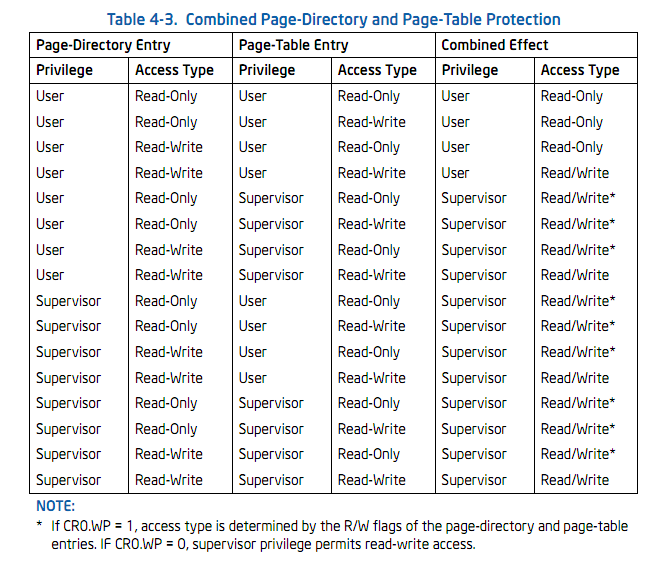
\includegraphics[scale=0.50]{/home/zhangchi/lab/report/screen.png}
\end{figure}

这个图应该是很容易看明白的,只有一个不太清楚的地方,就是为什么当最终组合效果的权限要求是内核态时,读写权限全部是可读也可写的?

助教告诉我,因为在内核态下,内核想要写入任意地址都是可行的。即便内核在写入一个表项时发现该页表项权限只能允许它读的话,通过修改CR0.WP寄存器,内核也能最终写入这个地址,所以访问类型就显得没有意义了,感谢张顺廷师兄的解释!!

接下来看看要填的第二个函数\funcname{boot\_map\_segment()}:



\begin{lstlisting}[style=ccode, title={\scriptsize \ttfamily \bfseries kern/pmap.c: boot\_map\_segment ()}]
static void
boot_map_segment(pde_t *pgdir, uintptr_t la, size_t size, physaddr_t pa, int perm)
{
    int offset;
    pte_t *pte;

    for (offset = 0; offset < size; offset += PGSIZE) {
        pte = pgdir_walk (pgdir, (void*)la, 1);

        *pte = pa|perm|PTE_P;

        pa += PGSIZE;
        la += PGSIZE;
    }
}
\end{lstlisting}

这个函数的作用是将线性地址la开始的size大小的区域映射到物理页面pa开始的同样大小区域。代码很直接,没什么好说的。实现完这个函数后,我们可以回到\funcname{i386\_vm\_init ()}从上次停下的地方继续往下看:\label{addrmapping}



\begin{lstlisting}[style=ccode, title={\scriptsize \ttfamily \bfseries kern/pmap.c: i386\_vm\_init ()}]
	//////////////////////////////////////////////////////////////////////
	// Now we set up virtual memory 
	
	//////////////////////////////////////////////////////////////////////
	// Map 'pages' read-only by the user at linear address UPAGES
	// Permissions:
	//    - the new image at UPAGES -- kernel R, user R
	//      (ie. perm = PTE_U | PTE_P)
	//    - pages itself -- kernel RW, user NONE
	// Your code goes here:
	boot_map_segment (
            pgdir, 
            UPAGES, 
            ROUNDUP (npage * sizeof (struct Page), PGSIZE), 
            PADDR ((uintptr_t) pages), // PADDR returns a (void*)
            PTE_U);

	//////////////////////////////////////////////////////////////////////
	// Use the physical memory that 'bootstack' refers to as the kernel
	// stack.  The kernel stack grows down from virtual address KSTACKTOP.
	// We consider the entire range from [KSTACKTOP-PTSIZE, KSTACKTOP) 
	// to be the kernel stack, but break this into two pieces:
	//     * [KSTACKTOP-KSTKSIZE, KSTACKTOP) -- backed by physical memory
	//     * [KSTACKTOP-PTSIZE, KSTACKTOP-KSTKSIZE) -- not backed; so if
	//       the kernel overflows its stack, it will fault rather than
	//       overwrite memory.  Known as a "guard page".
	//     Permissions: kernel RW, user NONE
	// Your code goes here:
	//
	boot_map_segment (
            pgdir,
            KSTACKTOP - KSTKSIZE,
            KSTKSIZE, // 8 * PGSIZE
            PADDR ((uintptr_t) bootstack),
            PTE_W);

	//////////////////////////////////////////////////////////////////////
	// Map all of physical memory at KERNBASE. 
	// Ie.  the VA range [KERNBASE, 2^32) should map to
	//      the PA range [0, 2^32 - KERNBASE)
	// We might not have 2^32 - KERNBASE bytes of physical memory, but
	// we just set up the mapping anyway.
	// Permissions: kernel RW, user NONE
	// Your code goes here: 
        boot_map_segment (
            pgdir,
            KERNBASE,
            ~KERNBASE + 1, 
            // 2^32 - KERNBASE = (2 ^ 32 - 1 - KERNBASE) + 1 = ~KERNBASE + 1
            (physaddr_t) 0,
            PTE_W); 
\end{lstlisting}

其中最后一段就是映射的KERNBASE以上的虚拟空间到物理地址操作系统本身。这个是为了将来打开页式转换以后操作系统也能使用统一的虚拟地址来访问其自身的数据。

按照注释的指示设置好映射关系即可,唯一需要留意的地方就是传参数的时候记住将内核虚拟地址的变量都用uintptr\_t转换一下类型。

接下来的几个函数都不是很难:\funcname{page\_lookup ()} 查找一个虚拟地址对应的具体Page:

\begin{lstlisting}[style=ccode, title={\scriptsize \ttfamily \bfseries kern/pmap.c: page\_lookup ()}]
struct Page *
page_lookup(pde_t *pgdir, void *va, pte_t **pte_store)
{
    pte_t *pte = pgdir_walk (pgdir, va, 0);

    if (pte_store != 0) {
        *pte_store = pte;
    }

    if (pte != NULL && (*pte & PTE_P)) {
        return pa2page (PTE_ADDR (*pte));
    }
    
	return NULL;
}
\end{lstlisting}

\funcname{page\_lookup ()} 在页目录中删除一个虚拟地址对应的二级页表表项。

\begin{lstlisting}[style=ccode, title={\scriptsize \ttfamily \bfseries kern/pmap.c: page\_remove ()}]
void
page_remove(pde_t *pgdir, void *va)
{
    pte_t *pte;
    struct Page *physpage = page_lookup (pgdir, va, &pte);

    if (physpage != NULL) {
        page_decref (physpage);
        *pte = 0;
        tlb_invalidate (pgdir, va);
    }
}
\end{lstlisting}

还有\funcname{page\_insert () }:

\begin{lstlisting}[style=ccode, title={\scriptsize \ttfamily \bfseries kern/pmap.c: boot\_alloc ()}]
int
page_insert(pde_t *pgdir, struct Page *pp, void *va, int perm) 
{
    pte_t *pte = pgdir_walk (pgdir, va, 1);

    if (pte == NULL) {
        return -E_NO_MEM;
    }

    if (*pte & PTE_P) {
        if (PTE_ADDR(*pte) == page2pa (pp)) {
            tlb_invalidate (pgdir, va);
            pp -> pp_ref --;
        } else {
            page_remove (pgdir, va);
        }
    }
    
    *pte = page2pa (pp)|perm|PTE_P;
    pp -> pp_ref ++;

    return 0;
}
\end{lstlisting}

这个函数负责将一个虚拟地址映射到它实际对应的物理页面上去,这里有几种调用的情况:

\begin{enumerate}
\item{这个虚拟地址所在地址在二级页表上没有挂载页面,那么这时直接修改相应的二级页表表项即可}
\item{如果已经挂载了页面,且页面和当前分配的物理页面不一样,那么就卸下原来的页面,再挂载新的页面。}
\item{如果已经挂载了页面,而且已挂载页面和当前分配的物理页面是同样的,这是什么情况呢?这种情况非常普遍,就是当内核要修改一个页面的访问权限时,它会将同一个页面重新插入一次,传入不同的perm参数,即完成了权限修改。}
\end{enumerate}

所以注意第13行代码,修改权限并没有增加一个物理页面的引用数目,所以这里先减了1,方便后面加回来。第12行代码重置了TLB但第15行没有,因为\funcname{page\_remove ()}函数中已经将移除的物理页自动重置TLB了,这里就没有必要重复清空了。

至此,我们已经把所有要求的函数填完了,重新编译运行JOS,连同page\_check() 和 check\_boot\_pgdir() 应该都可以通过了。即我们提前把Part 3的内容也做完了。如命令行打印:

\begin{lstlisting}[style=console]
6828 decimal is 15254 octal!
Physical memory: 66556K available, base = 640K, extended = 65532K
check_page_alloc() succeeded!
page_check() succeeded!
check_boot_pgdir() succeeded!
Welcome to the JOS kernel monitor!
Type 'help' for a list of commands.
K> 
\end{lstlisting}


\section{Kernel Address Space}

\subsection{Permissions and Fault Isolation}

关于$[\mathrm{UTOP},\mathrm{ULIM})$的空间我们早已讨论过。

\subsection{Initializing the Kernel Address Space}

\begin{lstlisting}[style=exercise]
|Exercise 5|. Fill in the missing code in i386_vm_init() after the call to page_check().

Your code should now pass the check_boot_pgdir() check.
\end{lstlisting}
已完成

\vspace{2em}

\begin{lstlisting}[style=exercise]
|Question|

|1.| What entries (rows) in the page directory have been filled in at this point? What addresses do they map and where do they point? In other words, fill out this table as much as possible:
|Entry|	|Base Virtual Address|    |Points to (logically):|
1023	?	                Page table for top 4MB of phys memory
1022	?	                ?
.	?	                ?
.	?	                ?
.	?	                ?
2	0x00800000	        ?
1	0x00400000	        ?
0	0x00000000	        [see next question]

|2.| After check_boot_pgdir(), i386_vm_init() maps the first four MB of virtual address space to the first four MB of physical memory, then deletes this mapping at the end of the function. Why is this mapping necessary? What would happen if it were omitted? Does this actually limit our kernel to be 4MB? What must be true if our kernel were larger than 4MB?
|3.| (From Lecture 4) We have placed the kernel and user environment in the same address space. Why will user programs not be able to read or write the kernel's memory? What specific mechanisms protect the kernel memory
|4.| What is the maximum amount of physical memory that this operating system can support? Why?
|5.| How much space overhead is there for managing memory, if we actually had the maximum amount of physical memory? How is this overhead broken down?
\end{lstlisting}

\vspace{2em}
\hrule
\vspace{2em}

\label{osmemarea}

\begin{enumerate}
\item{具体的虚拟地址到物理地址的映射关系在\ref{addrmapping}中已经结合JOS代码详细解释过了}
\item{我们来看看那段代码具体是如何作的:
\begin{lstlisting}[style=ccode, title={\scriptsize \ttfamily \bfseries kern/pmap.c: i386\_vm\_init ()}]
	//////////////////////////////////////////////////////////////////
	// On x86, segmentation maps a VA to a LA (linear addr) and
	// paging maps the LA to a PA.  I.e. VA => LA => PA.  If paging is
	// turned off the LA is used as the PA.  Note: there is no way to
	// turn off segmentation.  The closest thing is to set the base
	// address to 0, so the VA => LA mapping is the identity.

	// Current mapping: VA KERNBASE+x => PA x.
	//     (segmentation base=-KERNBASE and paging is off)

	// From here on down we must maintain this VA KERNBASE + x => PA x
	// mapping, even though we are turning on paging and reconfiguring
	// segmentation.

	// Map VA 0:4MB same as VA KERNBASE, i.e. to PA 0:4MB.
	// (Limits our kernel to <4MB)
	pgdir[0] = pgdir[PDX(KERNBASE)];

	// Install page table.
	lcr3(boot_cr3);

	// Turn on paging.
	cr0 = rcr0();
	cr0 |= CR0_PE|CR0_PG|CR0_AM|CR0_WP|CR0_NE|CR0_TS|CR0_EM|CR0_MP;
	cr0 &= ~(CR0_TS|CR0_EM);
	lcr0(cr0);

	// Current mapping: KERNBASE+x => x => x.
	// (x < 4MB so uses paging pgdir[0])

	// Reload all segment registers.
	asm volatile("lgdt gdt_pd");
	asm volatile("movw %%ax,%%gs" :: "a" (GD_UD|3));
	asm volatile("movw %%ax,%%fs" :: "a" (GD_UD|3));
	asm volatile("movw %%ax,%%es" :: "a" (GD_KD));
	asm volatile("movw %%ax,%%ds" :: "a" (GD_KD));
	asm volatile("movw %%ax,%%ss" :: "a" (GD_KD));
	asm volatile("ljmp %0,$1f\n 1:\n" :: "i" (GD_KT));  // reload cs
	asm volatile("lldt %%ax" :: "a" (0));

	// Final mapping: KERNBASE+x => KERNBASE+x => x.

	// This mapping was only used after paging was turned on but
	// before the segment registers were reloaded.
	pgdir[0] = 0;

	// Flush the TLB for good measure, to kill the pgdir[0] mapping.
	lcr3(boot_cr3);
}
\end{lstlisting}

这段代码中顺序有这么几个主要的操作:
\begin{itemize}
\item{第17行到第26行:重置页目录的第一项,并打开页表转换机制,\highlight{在这个之前,没有页式地址转换},所以所有的虚拟地址经过一次段地址转换就直接得到物理地址了,即paddr $=$ laddr $=$ vaddr $-$ KERNBASE,laddr 到 paddr 是等价的。在这个之后,线性地址laddr到物理地址paddr的页式转换打开。注意,这个时候,\highlight{会操作内存的程序只有内核},而内核访问内存的地址都是内核虚拟地址($\geq$KERNBASE),且这个时候页表的第一项pgdir[0]被设置成了pgdir[PDX[KERNBASE]],所以任意一个内核访问vaddr$=$KERNBASE $+$ x都先经过一次段式转换得到laddr $=$ vaddr $-$ KERNBASE $=$ x,然后laddr经过页式转换实际上等价于访问原来虚拟地址KERNBASE上面的同样地址,所以还是访问到内核自己的东西。把pgdir[0]重设的目的就是让内核地址在打开页式转换以后仍然能找到其自己所在的位置,因为后面如第33行内联汇编代码需要使用到内核中定义的常量GD\_UD等,内核在引用它们时都是使用的虚拟地址。}
\item{第32行到39行:关闭段式地址转换,即把原来是-KERNBASE的段基址赋值为零即可。这个时候一个内核虚拟地址KERNBASE$+$x转化为的线性地址laddr就是KERNBASE $+$ x本身,那么这个时候进入页式转换,查找到的就是内核其自身的物理地址,这个前面已经解释过了。}
\item{第45到第48行:内核已经能通过关闭段式转换只依靠页式转换实现正常访问其自身了,那么这时虚拟地址的低4MB的设置已经没用,需要还原清空,然后重置TLB}
\end{itemize}
}

\item{用户当然不能写内核地址的数据\ldots,这个问题不予回答}
\item{这个问题我们在前面已经分析过了,其中UPAGES存放的是系统pages的空间,系统分配的虚拟空间是PTSIZE,对应能管理的实际物理内存大概是1.3G左右}
\item{管理物理内存实际的内存开销为1个页目录+1024个页表,即1025 $\times$ 4KB大概为4MB的样子。}
\end{enumerate}

\vspace{4em}

\begin{lstlisting}[style=challenge]
|Challenge!| We consumed many physical pages to hold the page tables for the KERNBASE mapping. Do a more space-efficient job using the PTE_PS ("Page Size") bit in the page directory entries. This bit was not supported in the original 80386, but is supported on more recent x86 processors. You will therefore have to refer to Volume 3 of the current Intel manuals. Make sure you design the kernel to use this optimization only on processors that support it!
\end{lstlisting}

\vspace{4em}

根据查询x86手册的{\ttfamily \bfseries CHAPTER 3 PROTECTED-MODE MEMORY MANAGEMENT} 中 {\ttfamily \bfseries 3.6 PAGING (VIRTUAL MEMORY) OVERVIEW} 可以查到,如果将CR4中的PSE位打开,那么就可以开启4MB物理页。那么对应使用该物理页的虚拟地址寻址方式变为:

\vspace{4em}

\begin{figure}[htp]
\centering
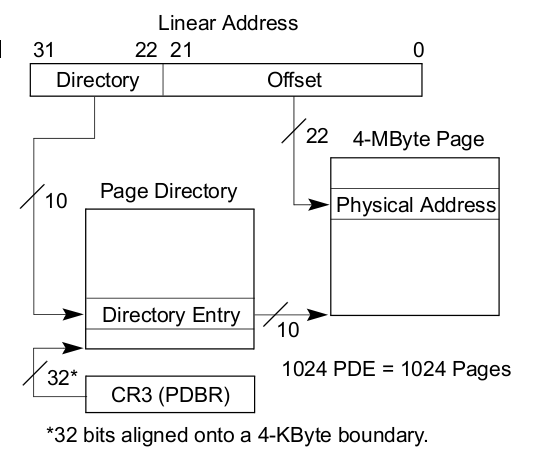
\includegraphics[scale=0.40]{/home/zhangchi/lab/report/screen3.png}
\end{figure}

这个时候相应的页目录表项也要修改,要修改其PS位表明该表项对应的地址是4MB,不用再进行二级页表寻址了:

\begin{figure}[htp]
\centering
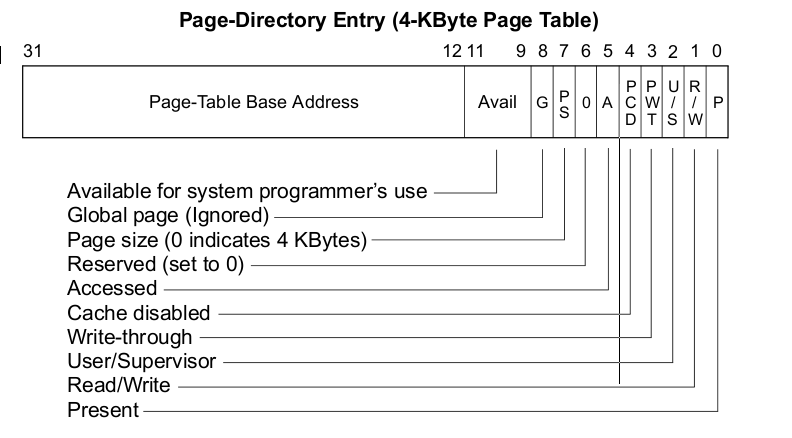
\includegraphics[scale=0.40]{/home/zhangchi/lab/report/screen4.png}
\end{figure}

但是这个时候会出现一个问题,就是设置了使用4MB页表以后,我们在前面程序中使用的那些二级页表查找和插入的过程就不能通用了,或者说都要相应的修改,比如\funcname{pgdir\_walk ()}, \funcname{page\_insert ()}等等。因为在后面的challenge中会要求提供命令手动对地址映射进行相应的修改和查询,所以为了简单,我没有把这个challenge和后面的结合起来,只是作为一个branch写了出来。相应的代码就是在kern/pmap.c中修改KERNBASE的地址映射时使用一个特别的映射过程:

\begin{lstlisting}[style=ccode, title={\scriptsize \ttfamily \bfseries kern/pmap.c: boot\_map\_KERNBASE ()}]
}
//
// Added by Chi Zhang (zhangchitc@gmail.com)
// Use 4MB page mapping for KERNBASE space

static void
boot_map_KERNBASE (pde_t *pgdir)
{
    uint32_t offset;
    uint32_t nspace = (~KERNBASE + 1);
    uint32_t pagesz = PTSIZE;
    uintptr_t la = KERNBASE;

    pde_t *pde;

    for (offset = 0; offset < nspace; offset += pagesz) {

        pde = pgdir + PDX(la);
        *pde = PADDR (la)|PTE_PS|PTE_W|PTE_P;
       
        la += pagesz;
    }
}
\end{lstlisting}

然后在打开页式转换之前重设CR4:


\begin{lstlisting}[style=ccode, title={\scriptsize \ttfamily \bfseries kern/pmap.c: i386\_vm\_init ()}]
        //
        // Added by Chi Zhang (zhangchitc@gmail.com)
        // Turn on CR4_PSE for 4MB page
        lcr4 (rcr4 () | CR4_PSE);
	
	// Map VA 0:4MB same as VA KERNBASE, i.e. to PA 0:4MB.
	// (Limits our kernel to <4MB)
	pgdir[0] = pgdir[PDX(KERNBASE)];

	// Install page table.
	lcr3(boot_cr3);

	// Turn on paging.
	cr0 = rcr0();
	cr0 |= CR0_PE|CR0_PG|CR0_AM|CR0_WP|CR0_NE|CR0_TS|CR0_EM|CR0_MP;
        cr0 &= ~(CR0_TS|CR0_EM);
        lcr0(cr0);
\end{lstlisting}

注意一点,这个时候对KERNBASE区域的二级寻址就失败了,因为在\funcname{check\_boot\_pgdir()} 有相应的KERNBASE的寻址检查,这样这个检查我们就通不过了,不过没有关系,如果页表设置正确,那么在打开4MB物理页以后,内核能正确完成kern/pmap.c接下来的基本寄存器重设的话,那么肯定寻址就是正确的,所以我们在\funcname{i386\_vm\_init()}的最后添加一条打印语句:

\begin{lstlisting}[style=ccode, title={\scriptsize \ttfamily \bfseries kern/pmap.c: i386\_vm\_init ()}]
	// Current mapping: KERNBASE+x => x => x.
	// (x < 4MB so uses paging pgdir[0])

	// Reload all segment registers.
	asm volatile("lgdt gdt_pd");
	asm volatile("movw %%ax,%%gs" :: "a" (GD_UD|3));
	asm volatile("movw %%ax,%%fs" :: "a" (GD_UD|3));
	asm volatile("movw %%ax,%%es" :: "a" (GD_KD));
	asm volatile("movw %%ax,%%ds" :: "a" (GD_KD));
	asm volatile("movw %%ax,%%ss" :: "a" (GD_KD));
	asm volatile("ljmp %0,$1f\n 1:\n" :: "i" (GD_KT));  // reload cs
	asm volatile("lldt %%ax" :: "a" (0));

	// Final mapping: KERNBASE+x => KERNBASE+x => x.

	// This mapping was only used after paging was turned on but
	// before the segment registers were reloaded.
	pgdir[0] = 0;

	// Flush the TLB for good measure, to kill the pgdir[0] mapping.
	lcr3(boot_cr3);

    cprintf ("4MB pages for KERNBASE space set up successfully!\n");
}

\end{lstlisting}

启动JOS我们发现成功的打印了这条语句:

\begin{figure}[htp]
\centering
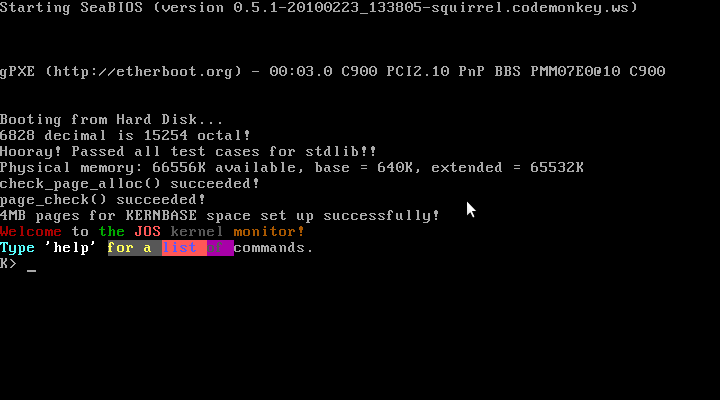
\includegraphics[scale=0.40]{/home/zhangchi/lab/report/screen-QEMU.png}
\end{figure}


\vspace{4em}


\begin{lstlisting}[style=challenge]
|Challenge!| Extend the JOS kernel monitor with commands to:

* Display in a useful and easy-to-read format all of the physical page mappings (or lack thereof) that apply to a particular range of virtual/linear addresses in the currently active address space. For example, you might enter 'showmappings 0x3000 0x5000' to display the physical page mappings and corresponding permission bits that apply to the pages at virtual addresses 0x3000, 0x4000, and 0x5000.
* Explicitly set, clear, or change the permissions of any mapping in the current address space.
* Dump the contents of a range of memory given either a virtual or physical address range. Be sure the dump code behaves correctly when the range extends across page boundaries!
* Do anything else that you think might be useful later for debugging the kernel. (There's a good chance it will be!)
\end{lstlisting}

\begin{enumerate}
\item{打印地址映射只需要调用kern/pmap.c中相应的\funcname{pgdir\_walk ()}过程就可以实现相应的查找

\begin{lstlisting}[style=ccode, title={\scriptsize \ttfamily \bfseries kern/monitor.c}]
int 
showmappings (uint32_t lva, uint32_t uva)
{    
    pte_t *pte;
    
    while (lva < uva) {
        pte = pgdir_walk (boot_pgdir, (void*) lva, 0);

        cprintf ("0x%x - 0x%x     ", lva, lva + PGSIZE);

        if (pte == NULL || !(*pte & PTE_P)) {
            cprintf ("not mapped\n");
        } else {
            cprintf ("0x%x   ", PTE_ADDR (*pte));

            if (*pte & PTE_U) 
                cprintf ("user: ");
            else
                cprintf ("kernel: ");
            
            if (*pte & PTE_W) 
                cprintf ("read/write");
            else
                cprintf ("read only");

            cprintf ("\n");
        }

        lva += PGSIZE;
    }
 
    return 0;
}

int
mon_showmappings (int argc, char **argv, struct Trapframe *tf)
{
    if (argc != 3) {
        cprintf ("Usage: showmappings [LOWER_ADDR] [UPPER_ADDR]\n");
        cprintf ("Both address must be aligned in 4KB\n");
        return 0;
    }

    uint32_t lva = strtol (argv[1], 0, 0);
    uint32_t uva = strtol (argv[2], 0, 0);

    if (lva != ROUNDUP (lva, PGSIZE) ||
        uva != ROUNDUP (uva, PGSIZE) ||
        lva > uva) {
        cprintf ("showmappings: Invalid address\n");
        return 0;
    }

    showmappings (lva, uva);

    return 0;
}
\end{lstlisting}

测试的时候有三个地区可以看看,我们前面只做过三个地址的映射: UPAGES 、 KSTACKTOP 和 KERNBASE,我们看看UPAGES和KERNBASE:UPAGES地址为0xef7bc000,KERNBASE为0xf0000000:

\vspace{2em}

\begin{lstlisting}[style=console]
K> showmappings 0xef000000 0xef008000
0xef000000 - 0xef001000     0x118000   user: read only
0xef001000 - 0xef002000     0x119000   user: read only
0xef002000 - 0xef003000     0x11a000   user: read only
0xef003000 - 0xef004000     0x11b000   user: read only
0xef004000 - 0xef005000     0x11c000   user: read only
0xef005000 - 0xef006000     0x11d000   user: read only
0xef006000 - 0xef007000     0x11e000   user: read only
0xef007000 - 0xef008000     0x11f000   user: read only
K> showmappings 0xf0000000 0xf0004000
0xf0000000 - 0xf0001000     0x0   kernel: read/write
0xf0001000 - 0xf0002000     0x1000   kernel: read/write
0xf0002000 - 0xf0003000     0x2000   kernel: read/write
0xf0003000 - 0xf0004000     0x3000   kernel: read/write
K> 
\end{lstlisting}
}

\item{重设地址映射的一个要注意的地方就是:映射到的物理页面一定要是以前被其他虚拟地址映射过的。否则我们就必须通过\funcname{page\_alloc ()}函数拿相应的页面而不是强行指定。这样会造成物理页面分配的混乱。程序很简单,只需要调用相应的\funcname{page\_insert ()}函数即可

但是这里有一个非常纠结的地方,就是在JOS初始化的时候,我们唯一映射的三个空间UPAGES、 KSTACKTOP 和 KERNBASE 都是静态映射! 即他们映射的时候不改变物理页面的引用数。那么这个时候造成这个命令测试的困难,我的做法是测试之前人为先映射一个地址,测试完以后就删除:

\begin{lstlisting}[style=ccode, title={\scriptsize \ttfamily \bfseries kern/monitor.c}]
int
setmappings (uint32_t va, uint32_t memsize, uint32_t pa, int perm)
{
    uint32_t offset;

    for (offset = 0; offset < memsize; offset += PGSIZE) {
       page_insert (boot_pgdir, pa2page (pa + offset), (void *)va + offset, perm); 
    }

    return 0;
}

int
mon_setmappings (int argc, char **argv, struct Trapframe *tf)
{
    if (argc != 5) {
        cprintf ("Usage: setmappings [VIRTUAL_ADDR] [PAGE_NUM] [PHYSICAL_ADDR] [PERMISSION]\n");
        cprintf ("    Both virtual address and physical address must be aligned in 4KB\n");
        cprintf ("    Permission is one of 4 options ('ur', 'uw', 'kr', 'kw')\n");
        cprintf ("           u stands for user mode, k for kernel mode\n");

        cprintf ("\n     Make sure that the physical memory space has already been mounted before\n");
        return 0;
    }


    //
    // Added by Chi Zhang (zhangchitc@gmail.com)
    // Just for test use!!
    // In the beginning, there is no physical page mounted
    // (The KERNBASE above space is static mapping which did't affect the pp_ref
    // so we need manually insert a page
    // here I select the second physical page
    // 
    // page_insert (boot_pgdir, pages + 1, 0, 0);

    uint32_t va = strtol (argv[1], 0, 0);
    uint32_t pa = strtol (argv[3], 0, 0);
    uint32_t perm = 0;
    uint32_t memsize = strtol (argv[2], 0, 0) * PGSIZE;

    if (va != ROUNDUP (va, PGSIZE) ||
        pa != ROUNDUP (pa, PGSIZE) ||
        va > ~0 - memsize) {
        cprintf ("setmappings: Invalid address\n");
        return 0;
    }

    uint32_t offset;
    struct Page *pp;

    for (offset = 0; offset < memsize; offset += PGSIZE) {
        pp = pa2page (pa + offset);
        if (pp -> pp_ref == 0) {
            cprintf ("setmappings: Unmounted physical page: %x - %x\n", 
                pa + offset, pa + offset + PGSIZE);
            return 0;
        }
    }

    if (argv[4][0] == 'u') {
        perm |= PTE_U;
    }
    if (argv[4][1] == 'w') {
        perm |= PTE_W;
    }

    setmappings (va, memsize, pa, perm);

    cprintf ("Set memory mapping successfully!  The new mapping is:\n");
    showmappings (va, va + memsize);


    return 0;
}
\end{lstlisting}

测试的时候我们选择人为先映射第二个物理页到0地址上,然后再修改它:

\begin{lstlisting}[style=console]
K> QEMU 0.12.5 monitor - type 'help' for more information
(qemu) info pg
PDE(001) ef000000-ef400000 00400000 urw
 |-- PTE(000031) ef000000-ef031000 00031000 ur-
PDE(001) ef400000-ef800000 00400000 ur-
 |-- PTE(000001) ef7bc000-ef7bd000 00001000 urw
 |-- PTE(000001) ef7bd000-ef7be000 00001000 ur-
 |-- PTE(000001) ef7be000-ef7bf000 00001000 urw
 |-- PTE(000001) ef7bf000-ef7c0000 00001000 -rw
 |-- PTE(000040) ef7c0000-ef800000 00040000 urw
PDE(001) ef800000-efc00000 00400000 -rw
 |-- PTE(000008) efbf8000-efc00000 00008000 -rw
PDE(001) efc00000-f0000000 00400000 -rw
 |-- PTE(000001) effbc000-effbd000 00001000 urw
 |-- PTE(000001) effbd000-effbe000 00001000 ur-
 |-- PTE(000001) effbe000-effbf000 00001000 urw
 |-- PTE(000001) effbf000-effc0000 00001000 -rw
 |-- PTE(000040) effc0000-f0000000 00040000 urw
PDE(040) f0000000-00000000 10000000 urw
 |-- PTE(010000) f0000000-00000000 10000000 -rw
(qemu) fda
setmappings 0 1 4096 ur
Set memory mapping successfully!  The new mapping is:
0x0 - 0x1000     0x1000   user: read only
K> showmappings 0x0 0x2000
0x0 - 0x1000     0x1000   user: read only
0x1000 - 0x2000     not mapped
K> 

\end{lstlisting}

一开始的时候我们通过QEMU控制台看到并没有虚拟地址0x0的相应映射,执行setmappings后我们再用showmappings查看就有了。

}
\end{enumerate}









\begin{lstlisting}[style=ccode, title={\scriptsize \ttfamily \bfseries kern/pmap.c: i386\_vm\_init ()}]

\end{lstlisting}

\begin{lstlisting}[style=ccode, title={\scriptsize \ttfamily \bfseries kern/pmap.c: i386\_vm\_init ()}]

\end{lstlisting}


\begin{lstlisting}[style=console]
\end{lstlisting}

\begin{lstlisting}[style=console]
\end{lstlisting}
\begin{lstlisting}[style=console]
\end{lstlisting}

\begin{lstlisting}[style=console]
\end{lstlisting}
\begin{lstlisting}[style=console]
\end{lstlisting}

\begin{lstlisting}[style=console]
\end{lstlisting}
\subsection{Address Space Layout Alternatives}

\begin{lstlisting}[style=challenge]
|Challenge!| Write up an outline of how a kernel could be designed to allow user environments unrestricted use of the full 4GB virtual and linear address space. Hint: the technique is sometimes known as "follow the bouncing kernel." In your design, be sure to address exactly what has to happen when the processor transitions between kernel and user modes, and how the kernel would accomplish such transitions. Also describe how the kernel would access physical memory and I/O devices in this scheme, and how the kernel would access a user environment's virtual address space during system calls and the like. Finally, think about and describe the advantages and disadvantages of such a scheme in terms of flexibility, performance, kernel complexity, and other factors you can think of.
\end{lstlisting}

\begin{lstlisting}[style=challenge]
|Challenge!| Since our JOS kernel's memory management system only allocates and frees memory on page granularity, we do not have anything comparable to a general-purpose malloc/free facility that we can use within the kernel. This could be a problem if we want to support certain types of I/O devices that require physically contiguous buffers larger than 4KB in size, or if we want user-level environments, and not just the kernel, to be able to allocate and map 4MB superpages for maximum processor efficiency. (See the earlier challenge problem about PTE_PS.)
Generalize the kernel's memory allocation system to support pages of a variety of power-of-two allocation unit sizes from 4KB up to some reasonable maximum of your choice. Be sure you have some way to divide larger allocation units into smaller ones on demand, and to coalesce multiple small allocation units back into larger units when possible. Think about the issues that might arise in such a system.
\end{lstlisting}

\begin{lstlisting}[style=challenge]
|Challenge!| Extend the JOS kernel monitor with commands to allocate and free pages explicitly, and display whether or not any given page of physical memory is currently allocated. For example:

	K> alloc_page
		0x13000
	K> page_status 0x13000
		allocated
	K> free_page 0x13000
	K> page_status 0x13000
		free
	
Think of other commands or extensions to these commands that may be useful for debugging, and add them.
\end{lstlisting}

\begin{lstlisting}[style=ccode, title={\scriptsize \ttfamily \bfseries kern/pmap.c: i386\_vm\_init ()}]

\end{lstlisting}


\begin{lstlisting}[style=ccode, title={\scriptsize \ttfamily \bfseries kern/pmap.c: i386\_vm\_init ()}]
}
\end{lstlisting}

\begin{lstlisting}[style=ccode, title={\scriptsize \ttfamily \bfseries kern/pmap.c: i386\_vm\_init ()}]
}
\end{lstlisting}

\begin{lstlisting}[style=ccode, title={\scriptsize \ttfamily \bfseries kern/pmap.c: i386\_vm\_init ()}]
}
\end{lstlisting}

\begin{lstlisting}[style=console]
\end{lstlisting}

\begin{lstlisting}[style=console]
\end{lstlisting}


\clearpage

\end{CJK*}
\end{document}
	

e